\chapter{New ground-to-ground garden experiments and numerical analysis}
\section{What changed from the original report}
The general matrix-multiplication and matrix-exponential lessons have been
removed. Their instructional style is applied to the actual free-body equations,
linearization, transfer functions, full feedback polynomials and stability proofs.
The earlier known-map airborne test is retained as historical evidence. The new
experiment starts on the ground, takes off, navigates, approaches, descends and
lands with actual contact dynamics. Flight control still has exactly six PID
objects and the same angle/rate/vertical-speed interface.

The current boot gain candidate is $\lambda=0.7$, replacing the earlier
$\lambda=1$ default. This choice follows both the wider local stability checks
and a completed mission. It is a provisional simulation/bench candidate; it is
not a hardware flight tune. Host tests explicitly load their own gains when needed.
\section{Current six-controller candidate and model coefficients}
\begin{center}\begin{tabular}{lrrr}\toprule Controller & $K_p$ & $K_i$ & $K_d$\\\midrule
Roll angle & 3 & 0 & 0\\
Roll rate & 0.000829338154 & 0.0038702446 & 0\\
Pitch angle & 3 & 0 & 0\\
Pitch rate & 0.000829338154 & 0.0038702446 & 0\\
Yaw rate & 0.00537561392 & 0.008362066 & 0\\
Altitude & 0.108044997 & 0.0308699999 & 0.122500002\\
\bottomrule\end{tabular}\end{center}
Angular units are degrees and degrees/s, as in the C code. Normalized output
is a desired-thrust proxy. The assumed gains from allocation and mechanics are
$b_x=b_y=18231.40540218$ deg/s$^2$/command, $b_\psi=937.56730112$ deg/s$^2$/command, and $b_h=20$ m/s$^2$/command. The actuator lag is 0.04 s and translational drag rate is 0.1 s$^{-1}$.
For the conservative candidate, the following polynomials are
formed from the equations in the derivation chapters. They retain actuator lag;
height additionally retains drag. Write $T=N/D$ with descending powers:
\begin{align}
N_{\phi}(s)&=45.36s+211.68,\\
D_{\phi}(s)&=0.04 s^{4}+1s^{3}+15.12s^{2}+115.92s+211.68.
\end{align}
\begin{align}
N_{r}(s)&=5.04s+7.84,\\
D_{r}(s)&=0.04 s^{3}+1s^{2}+5.04s+7.84.
\end{align}
\begin{align}
N_{h}(s)&=2.45s^{2}+2.1609s+0.6174,\\
D_{h}(s)&=0.04 s^{4}+1.004s^{3}+2.55s^{2}+2.1609s+0.6174.
\end{align}
\section{Poles, step response, Routh values and sampling}
The table reports actual local transfer-function responses, including numerator
zeros. Settling means the last exit from a two-percent band over the simulated
20 s linear response; it is not a nonlinear aircraft landing time.
\begin{center}\small\begin{tabular}{llrrr}\toprule Scale & Loop & Overshoot [\%] & Settling [s] & Sampled radius\\\midrule
0.7 & angle & 0.000 & 1.385 & 0.9949320\\
0.7 & roll\_rate & 35.902 & 0.426 & 0.9863007\\
0.7 & yaw & 19.007 & 1.763 & 0.9938399\\
0.7 & height & 20.572 & 3.692 & 0.9986314\\
1 & angle & 0.000 & 1.344 & 0.9944676\\
1 & roll\_rate & 46.751 & 0.553 & 0.9846446\\
1 & yaw & 21.687 & 1.195 & 0.9908625\\
1 & height & 22.207 & 4.027 & 0.9979595\\
1.3 & angle & 0.000 & 1.325 & 0.9942743\\
1.3 & roll\_rate & 55.928 & 0.589 & 0.9867462\\
1.3 & yaw & 25.234 & 0.883 & 0.9900456\\
1.3 & height & 23.664 & 3.241 & 0.9973339\\
\bottomrule\end{tabular}\end{center}
The local continuous poles for the conservative loops are listed explicitly:
\begin{description}
\item[angle] $-5.89357+12.66510j,\ -5.89357-12.66510j,\ -10.67161+0.00000j,\ -2.54124+0.00000j$ s$^{-1}$.
\item[roll\_rate] $-9.00000+13.07670j,\ -9.00000-13.07670j,\ -7.00000+0.00000j$ s$^{-1}$.
\item[yaw] $-18.87451+0.00000j,\ -3.06274+1.00198j,\ -3.06274-1.00198j$ s$^{-1}$.
\item[height] $-22.35501+0.00000j,\ -1.37553+0.00000j,\ -0.68473+0.18192j,\ -0.68473-0.18192j$ s$^{-1}$.
\end{description}
The saved JSON contains full numerator/denominator arrays, every Routh first
column, phase margins for the rate loops, and sampled eigenvalues with and
without one flight-sample delay. The sixth-order horizontal models have positive
leading Hurwitz determinants for the tested candidates. Their multirate radii are:
\begin{center}\begin{tabular}{llrr}\toprule Scale & Guidance & 500 Hz/20 Hz radius & With 50 ms delay\\\midrule
0.7 & navigate & 0.9644378 & 0.9696527\\
0.7 & approach & 0.9522570 & 0.9552026\\
1 & navigate & 0.9654857 & 0.9708107\\
1 & approach & 0.9521239 & 0.9567542\\
1.3 & navigate & 0.9658711 & 0.9712471\\
1.3 & approach & 0.9520753 & 0.9573129\\
\bottomrule\end{tabular}\end{center}
These tests omit estimator states and map latency. They must not be confused
with proving real processor deadlines or global nonlinear stability.
\begin{figure}[htbp]\centering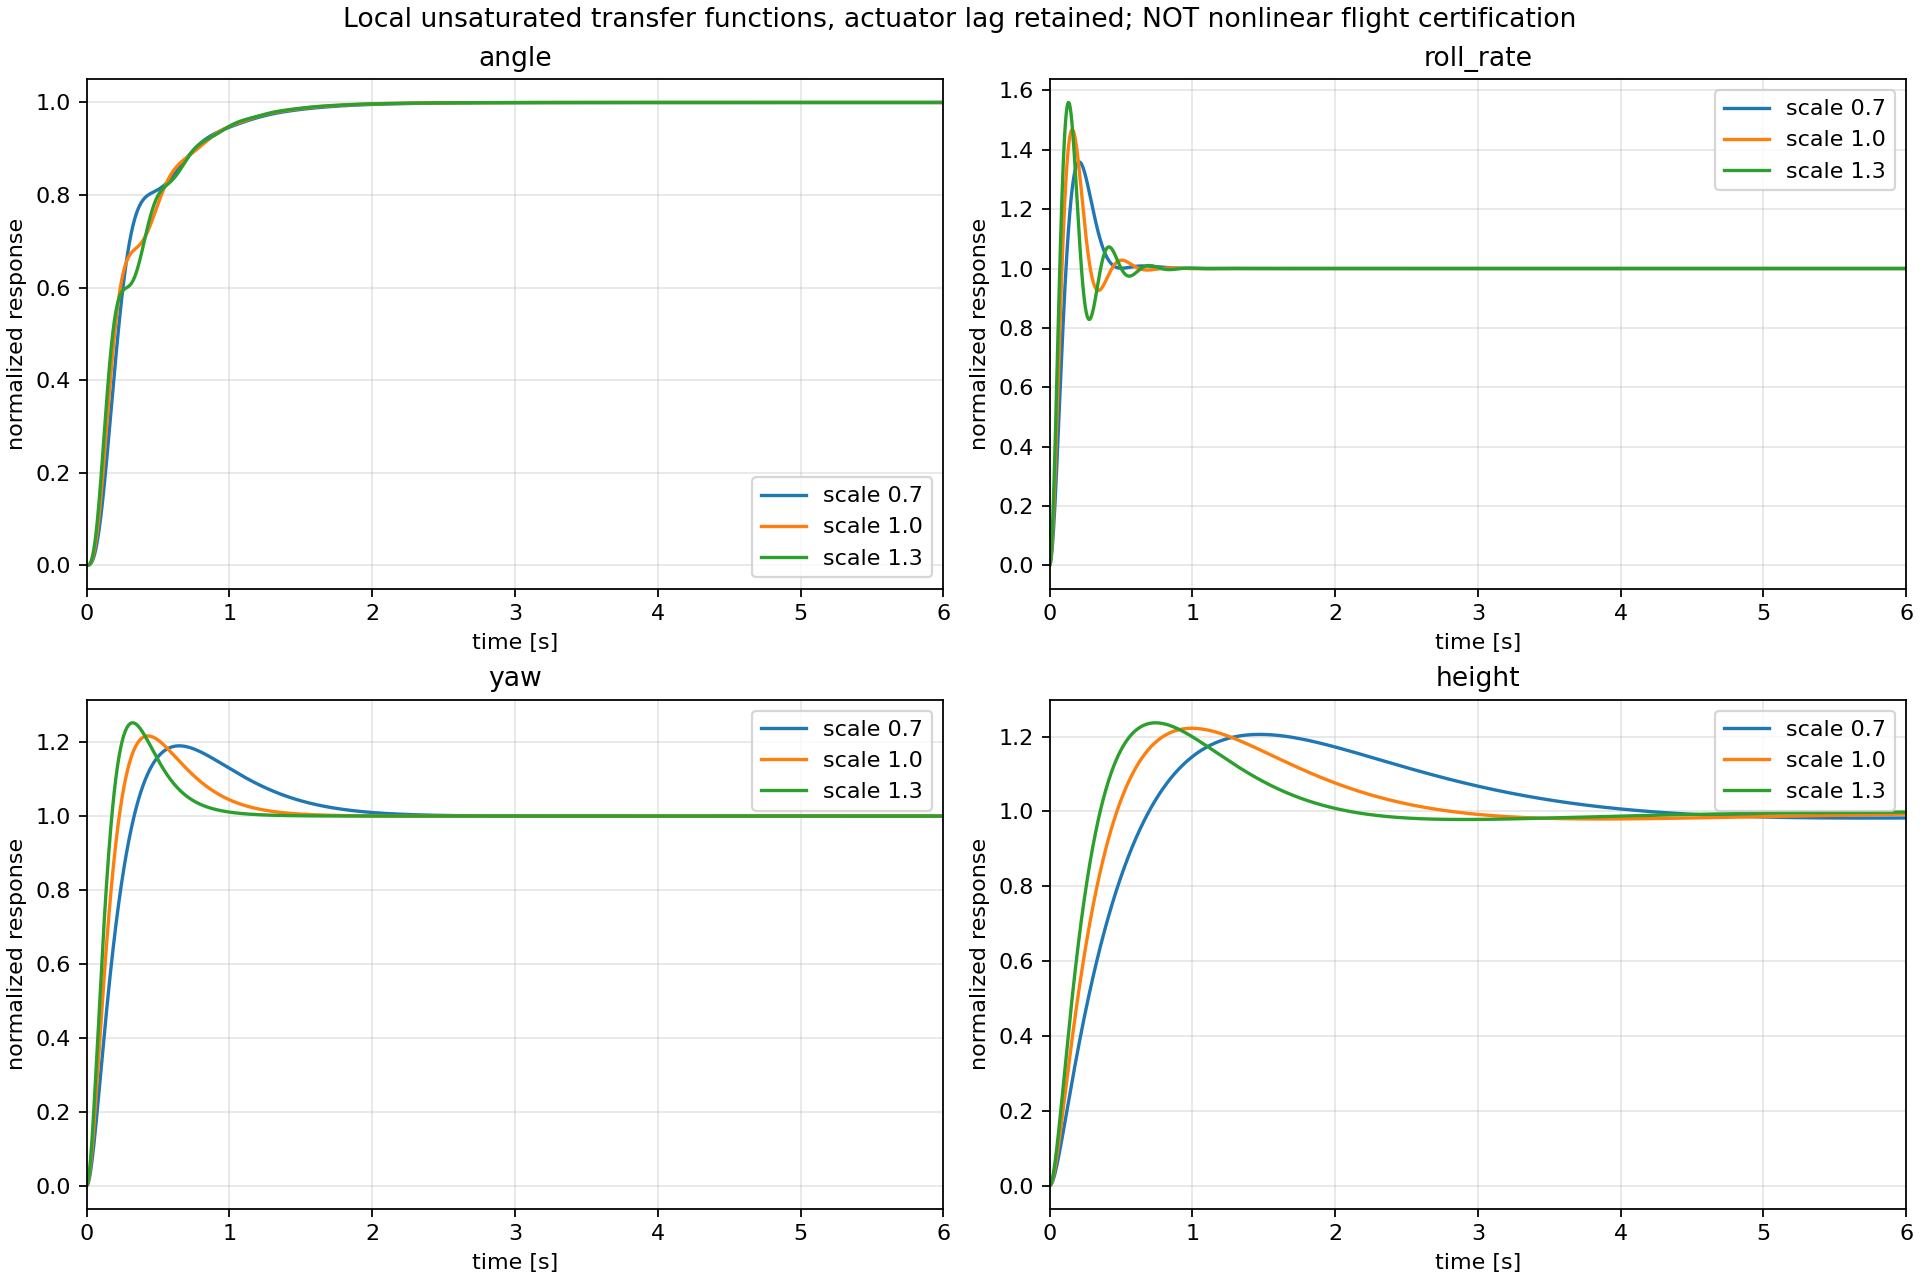
\includegraphics[width=\textwidth]{images/linear-step-responses.png}
\caption{Local transfer-function step responses. Overshoot differs from the nominal
second-order design because the complete models contain extra poles and zeros.}\end{figure}

\section{The uncertainty grid exposes a real tuning limitation}
The finite grid uses fifteen plant-gain factors from 0.65 to 1.35 and fifteen
actuator lags from 0.02 to 0.09s, for angle, yaw-rate and height models:
\begin{center}\begin{tabular}{lrrr}\toprule Scale & Stable tests & Total & Largest real pole\\\midrule
0.7 & 675 & 675 & -0.473717\\
1.0 & 673 & 675 & 0.069313\\
1.3 & 634 & 675 & 0.686074\\
\bottomrule\end{tabular}\end{center}
Thus the faster candidate is not robust over all these assumed points. The
separate analytic interval argument in the stability chapter proves the local
decoupled conservative-candidate inequalities throughout the stated continuous
box, including a height-drag interval. The complete camera-guided nonlinear
aircraft is not covered by that theorem. Actual motor lag remains unmeasured.

\section{Camera-only panel distance, derived from the measurement geometry}
The hardware direction is one RGB camera plus one downward 1D lidar. No depth
image is supplied to this planner. For this controlled course only, fixtures
are rectangular blue boards 1.2m wide and 1.8m high with white borders. Their
visible blue inner rectangle is 1.09m by 1.69m. These are chosen test-fixture
dimensions, not an assertion of a universal standard panel size.

YOLO identifies candidate image regions. Colour/contour fitting supplies four
ordered inner corners; clipped or nonconvex quadrilaterals are rejected. Given
calibrated intrinsics $K$, define planar object points
\begin{equation}
P_1=(-w/2,-H/2,0),\ P_2=(w/2,-H/2,0),\
P_3=(w/2,H/2,0),\ P_4=(-w/2,H/2,0).
\end{equation}
Each corner satisfies
\begin{equation}
\lambda_i\begin{bmatrix}u_i\\v_i\\1\end{bmatrix}=K(R_{CO}P_i+t_{CO}).
\end{equation}
The planar pose solver estimates $R_{CO},t_{CO}$. Positive depth and a
reprojection RMS below 2 pixels are required. A low reprojection error alone
does not prove correct metric scale or remove planar pose ambiguity.

In the frontal special case, apparent height $h_p$ pixels gives
$h_p=f_yH/Z$, so $Z=f_yH/h_p$. Differentiate this physical equation:
\begin{equation}
\frac{\partial Z}{\partial f_y}=\frac Z{f_y},\quad
\frac{\partial Z}{\partial H}=\frac ZH,\quad
\frac{\partial Z}{\partial h_p}=-\frac Z{h_p}.
\end{equation}
For independent small calibration/size/pixel errors,
\begin{equation}
\frac{\sigma_Z^2}{Z^2}\simeq
\frac{\sigma_f^2}{f_y^2}+\frac{\sigma_H^2}{H^2}+\frac{\sigma_p^2}{h_p^2}.
\end{equation}
This proves why distant small images have larger relative range uncertainty.
It also proves the unresolved scale problem: replacing both $H$ and $Z$ by
1.2 times their values leaves $h_p$ unchanged. A regression test explicitly
confirms that a 20\% wrong fixture size produces a 20\% wrong range scale.
The four rasterized geometry tests at 2.5--5 m have errors saved in the report;
they are synthetic calibration tests, not real camera accuracy measurements.

For the general four-corner fit, local pose covariance can be approximated by
$(J^{\mathsf T}\Sigma_{\rm pix}^{-1}J)^{-1}$ when the reprojection Jacobian has
sufficient rank and one pose solution dominates. A multimodal/ambiguous solution
must not be summarized as a single confident Gaussian. The implementation uses
a provisional conservative range scale $\sigma_r=0.04Z+0.03$m and obstacle
inflation; this heuristic is not a calibrated posterior covariance.

Optical right/down/forward transforms to body forward/left/up as
\begin{equation}(X_B,Y_B,Z_B)=(Z_C,-X_C,-Y_C).\end{equation}
Add the 0.18 m forward / 0.02 m upward camera lever arm, then use
$p_W=R_{WB}(p_B+t_{BC})+p_{WB}$.
World-map uncertainty also includes pose and extrinsic calibration errors;
simulated odometry supplies millimetre-scale translation noise and the true
orientation in this prototype. A real VIO implementation is still missing.

\section{Training and operating-domain limitations}
The actual YOLO11n derivative was trained for 12 epochs at 320 pixels on 180 synthetic
training images and 40 synthetic validation images. Validation poses are held out;
the simulation tests also change panel layouts. This is not a real-world
generalization test. Raw training output and its CSV are retained, including an
initial plotting-dependency error; the missing dependency was repaired later.
Real images, hard negatives, non-blue panels, lighting changes and unknown-size
objects remain unvalidated. No true obstacle coordinates, camera depth or
segmentation labels enter the online mapper. Renderer IDs are used only to
generate training labels, and true geometry is used only for offline scoring.

The downward ray lidar is a simulated range sensor, not a validated TOFSense
driver. On flat ground it supplies $h=(d+0.085)\cos\phi\cos\theta$ with a known
lever arm; invalid/near-ground returns are rejected. The C two-state height
filter corrects fresh lidar observations with variance 0.0004 m$^2$ in addition
to the barometer. Real surface reflectivity, slope, sunlight and sensor latency
have not been identified. Virtual ground contact is used by the mission's
touchdown confirmation; a reliable real landed detector remains unfinished.

\section{Recorded mission progression and outcomes}
The first attempt reached the ground without collision but missed the horizontal
finish by about 0.48 m and failed the 0.4 m criterion. Position feedback during
approach/landing fixed that problem. Later refinements require a stable approach
before descent, inhibit RT boost during approach/landing, and correct the visible
inner-panel dimensions. Earlier iteration files are preserved; not every early
iteration has a source hash. The delivery run records source hashes at startup.
\begin{center}\scriptsize\begin{tabular}{lrrrrl}\toprule Run & Time[s] & Final XY[m] & Clearance[m] & PnP obs & Result\\\midrule
initial-landing-drift & 35.35 & 0.47998 & 0.6998 & 37 & fail\\
garden-nominal & 35.35 & 0.05938 & 0.6998 & 37 & pass\\
garden-heldout & 32.05 & 0.03132 & 0.5597 & 44 & pass\\
garden-camera-dropout & 32.75 & 0.02545 & 0.7019 & 37 & pass\\
garden-boost-slew & 53.10 & 0.01703 & 0.4800 & 49 & pass\\
garden-conservative & 35.40 & 0.01896 & 0.5705 & 42 & pass\\
garden-selected-ros2 & 32.20 & 0.00792 & 0.3612 & 39 & pass\\
garden-final & 35.45 & 0.00814 & 0.4904 & 37 & pass\\
\bottomrule\end{tabular}\end{center}
Different layouts, seeds and software iterations are not a controlled speed
ranking. The delivered video selects the current conservative-gain, calibrated,
shared-C++ policy run with actual ROS 2 selection/transport, rather than claiming
a global optimum from those different courses. Boost can worsen mission settling;
it is an allowance, not evidence of better-than-FPV performance.
The delivery run takes 35.45s, ends 0.008137m from the requested XY finish, reaches 1.255538m and has minimum evaluated panel clearance 0.490441m including the conservative rotor-envelope collision shape. Height RMS error during hover/navigation/approach is 0.017921m, and height-estimation RMS error across the complete run is 0.003722m. These are conditional simulation values.
\begin{figure}[p]\centering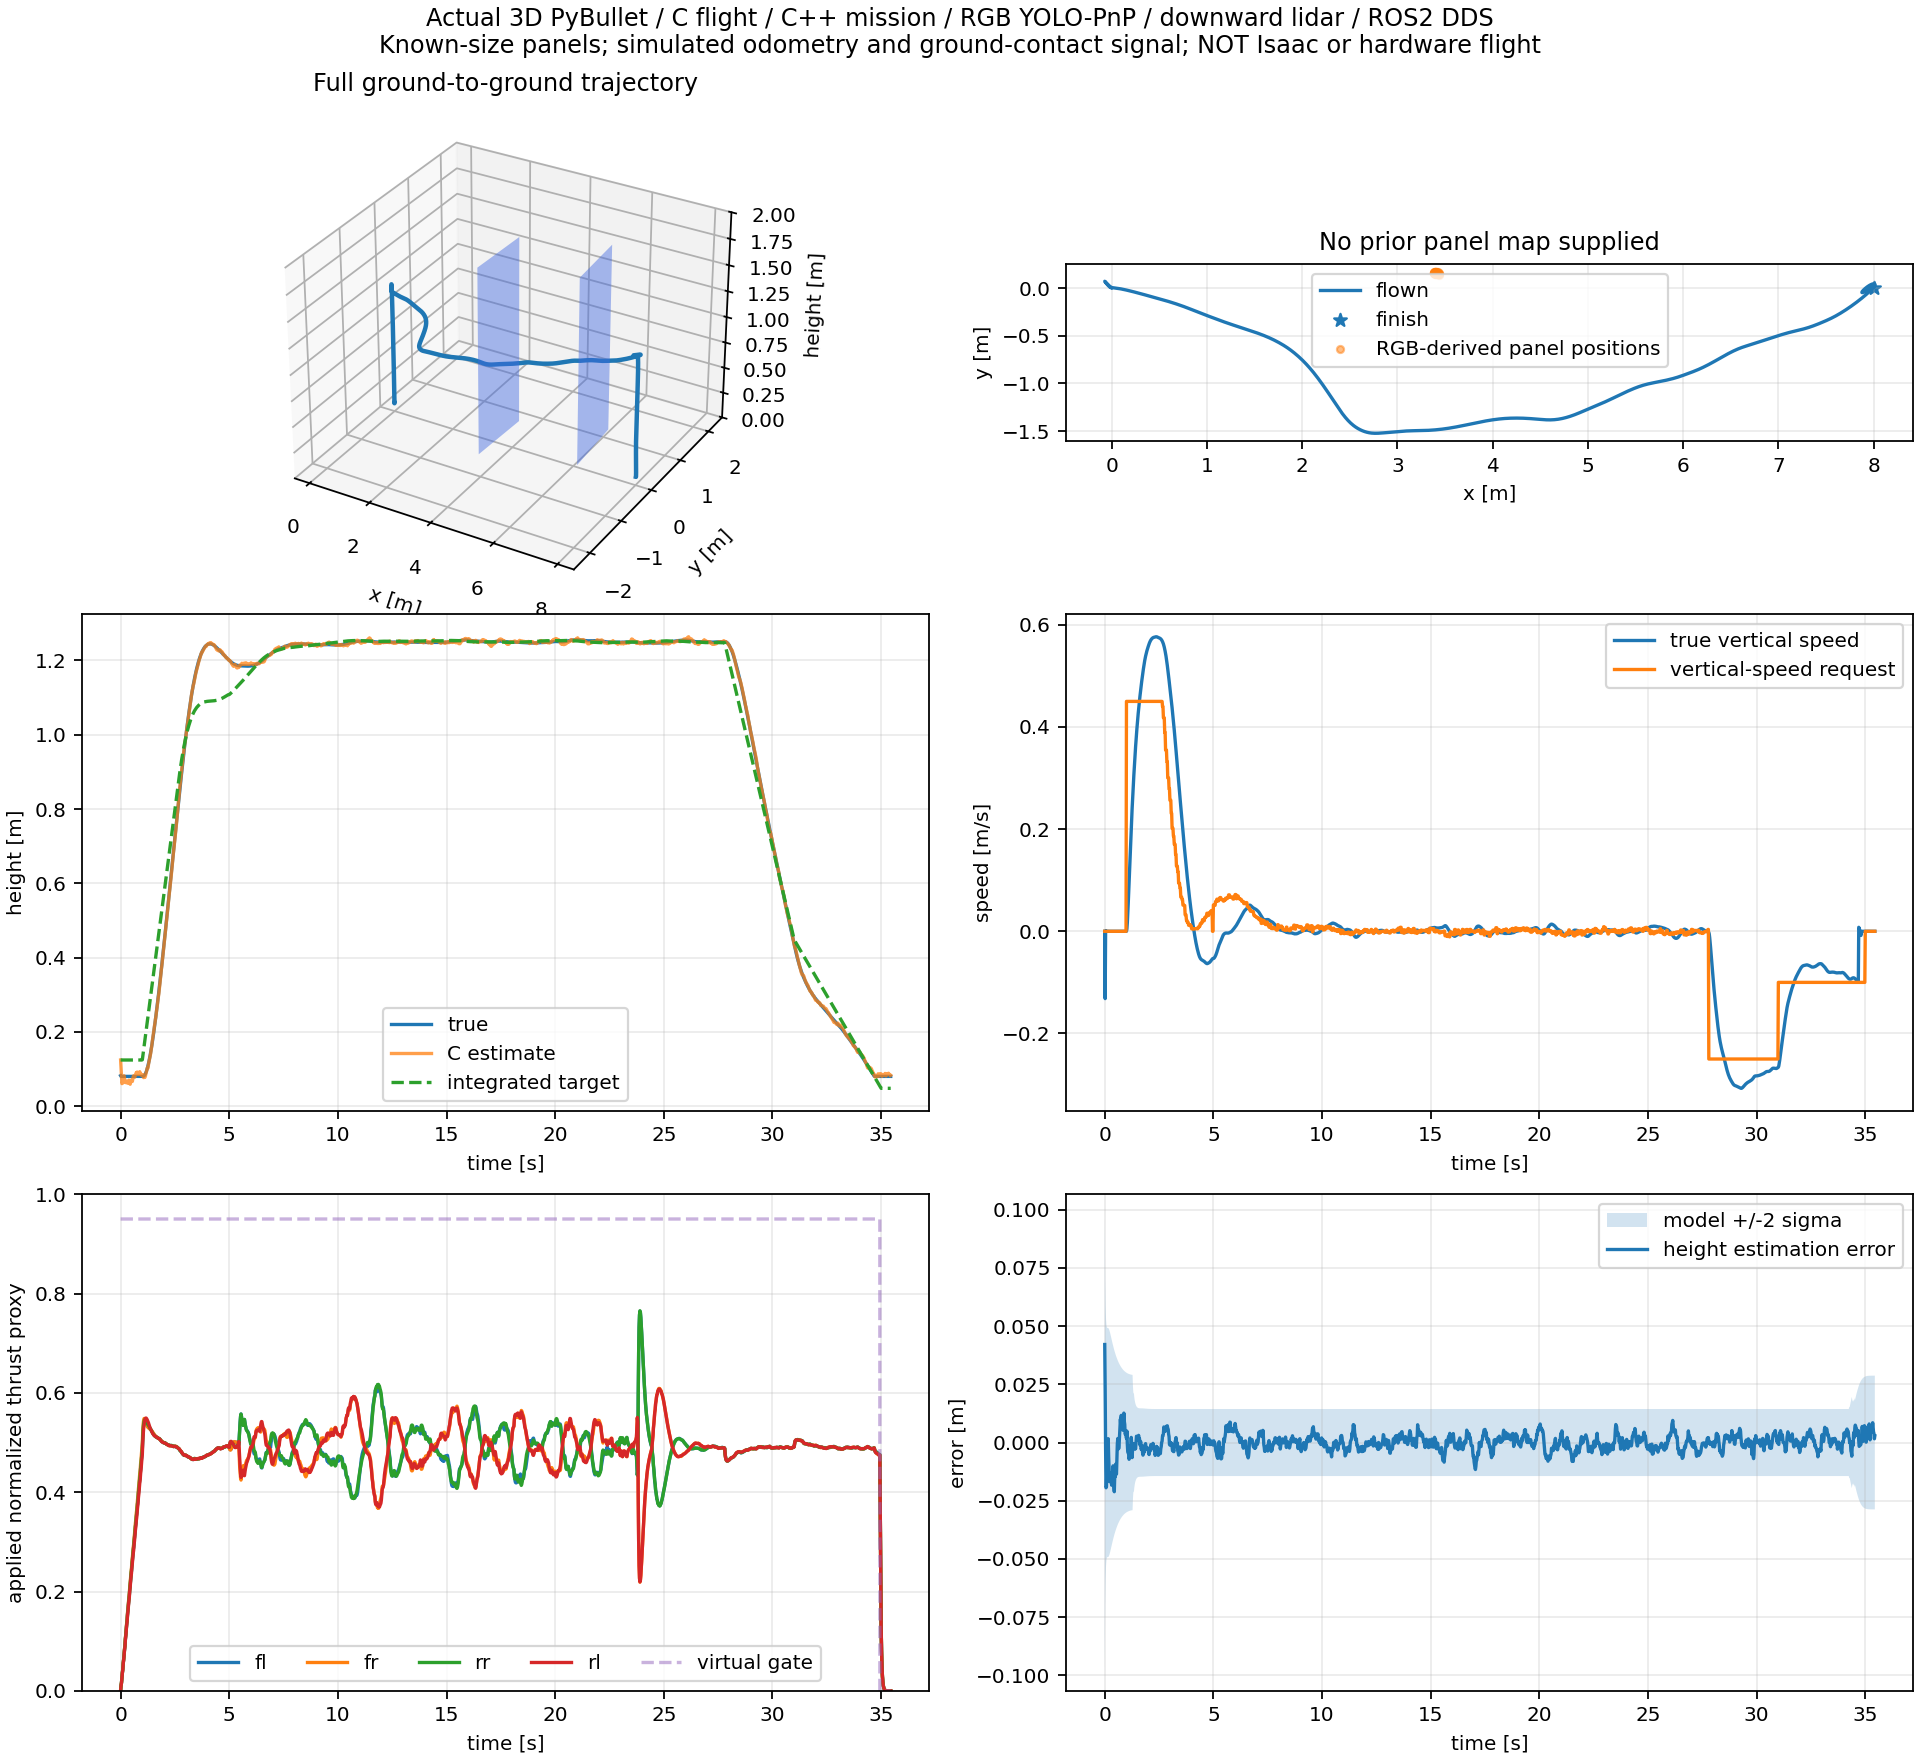
\includegraphics[width=\textwidth]{images/garden-final-graphs.png}
\caption{Original complete-flight data, including takeoff, landing and controller uncertainty.
True geometry shown in evaluation figures is not supplied to the online planner.}\end{figure}
\clearpage
\section{ROS 2 selection, timing and implementation boundaries}
The final adapter run completes 19,378 sequenced requests through two ROS 2 DDS nodes. Median measured request latency is 0.5113 ms, p99 is 1.5267ms and maximum is 22.9170 ms.
The test includes C resets,500 Hz control steps and lidar corrections.
A Python3.10 renderer reaches bundled Python3.12 ROS bindings through local
TCP IPC; DDS then carries the test request to the C subscriber and returns its
result. This is actual DDS execution, not proof that every Windows update meets
2  ms. The complete ROS C++ wrappers are authored but still unbuilt on this PC.

The working bundled selector accepts seven values: start XYZ, finish XYZ and
cruise height in local metres. ROS acknowledges the chosen values, and the
mission rejects a start that differs from the actual launch pose. The final
demonstration uses a separate initial-condition spawn, not an in-flight teleport.
The C++ package exposes RequestMission and a CLI client, plus a land-at-current-XY
request service. Camera PnP publishes metric observations into the online map.
No service, gesture or simulator gate enables physical motor arming.

\section{Current missing information and unresolved problems}
The separate project-status document orders the hardware questions. The main
remaining requirements are: measured takeoff mass/centre of mass/inertia;
motor/9047 thrust/current/lag data; exact ESC protocol; camera model and calibrated
intrinsics/extrinsics/timing; an implemented real local-pose/VIO source; exact
LoRa module/band and airtime budget; sensor drivers; routed PCB/power/current
measurement; real landed detection and tested sensor-loss/battery authority.
The garden is an original illustrative campus scene based on visual references,
not a surveyed USTHB map. Single RGB plus one lidar ray does not establish
general metric obstacle coverage without additional geometric assumptions or
validated motion-based reconstruction. Physical motors remain disabled.
